\documentclass[12pt,a4paper]{article}
\usepackage[utf8]{inputenc}
\usepackage{amsmath}
%\usepackage[brazilian]{babel} % Brazil or not Brazil??
\usepackage{amsfonts}
\usepackage{amssymb}
\usepackage{graphicx}
\usepackage[margin=0.8in]{geometry}


\begin{document}
\title{\vspace{70mm}\Huge Experimento 04 - Máquina de atwood}
\author{ Giovani Garuffi\qquad\hfill
		\textit {RA: 155559}\protect\\
		João Baraldi\hfill
		\textit{RA: 158044}\protect\\
		Lauro Cruz\hfill
		\textit{RA: 156175}\protect\\
		Lucas Schanner\hfill
		\textit{RA: 156412}\protect\\
		Pedro Stringhini\hfill
		\textit {RA: 156983}								
		}
\maketitle
\newpage
\section{Resumo}
Inicialmente, prendeu-se um fio (inextensível) com duas massas nas extremidades em uma polia em torno de um eixo fixo (Máquina de Atwood). Após variar a diferença entre as massas das extremidades dos pesos dos fios (com discos de metal de massas variadas) e obter os períodos de queda de da massa de maior peso com um cronômetro, foi utilizada a fórmula $\Delta m = (\dfrac{2h}{gR^2})(I + MR^2)\dfrac{1}{t^2}+(\dfrac{tau_a}{gR})$ para determinar o momento de inércia da polia e o torque do atrito.
Após a transformação linear da equação em $X$, traçou-se um gráfico de $\Delta m$ por $1/t^2$. A partir desses dados e das dimensões do cilindro (calculadas com um paquímetro), foi possível a determinação do momento de inércia aproximado e do torque realizado pela força de atrito na polia.
% Não me lembro das fórmulas e dos eixos do gráfico, sei q sou várzea, mas me ajudem ;) hahahaha

\section{Objetivos}
O experimento realizado teve como objetivo estudar a máquina de Atwood, utilizando para isso a determinação do momento de inércia da polia utilizada e do torque realizado pelo atrito entre tal polia e o fio que a toca.$T = \sqrt{\frac{8\pi I_0 L}{G r^4}}$


\section{Procedimento Experimental e Coleta de Dados}


\subsection{Procedimento}
A montagem do experimento da Máquina de Atwood consiste em dois pesos de suspensão ligados por um fio leve e inextensível (foi utilizado um pedaço de barabante), que passa por uma polia, um cilindro (no caso, um de latão de raio $R$, medido com o paquímetro, e momento de inércia $I$), como mostra a figura 1. \\

\newpage

\begin{figure}
\centering
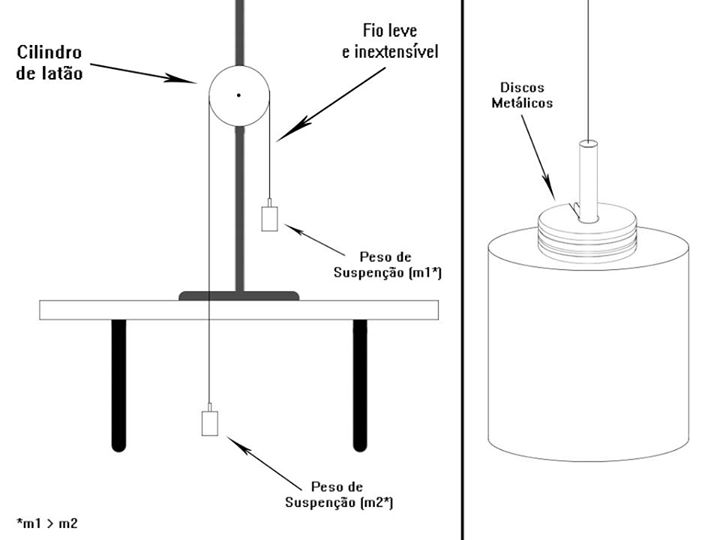
\includegraphics[scale=0.55]{FigUnica.jpg}
\caption{Montagem experimental}
\label{Fig1}
\end{figure}

Entre os pesos de suspensão, são distribuídos discos metálicos que aumentam sua massa total (vide figura 1). O objetivo desses discos é variar a massa em cada extremidade do fio, mas manter a soma $m1 + m2$ (vide figura 1) constante. Para tal, basta-se apenas passar os discos de um peso para o outro, para assim, dada a equação

$$\Delta m = (2h/gR^2)(I + MR^2)(1/t^2) + \tau_a/(gR),$$

apenas $\Delta m$, que é a diferença $m1 - m2$, mude, enquanto $M$, que é a soma $m1 + m2$, mantem-se constante.\\

O experimento em si consiste em abandonar o corpo mais pesado, $m1$, de uma altura $h$ constante, mensurada com a fita métrica, e medir o tempo $t$ de queda, com o cronômetro. Esse procedimento foi realizado três vezes e então foi tirado o tempo medio.

\subsection{Dados Obtidos}
As massas dos pesos de suspensão foram medidas, tais que

$$m1 = (891.6 \pm 0.1)g \;\; e \;\; m2 = (895.7 \pm 0.1)g$$

Já os discos têm massas de, em gramas:

\begin{table}[!htbp]
\centering
\caption{Massas dos discos metálicos}
\begin{tabular}{|c|c|c|c|c|c|c|c|}
\hline 
$m_{d1}$ & $m_{d2}$ & $m_{d3}$ & $m_{d4}$ & $m_{d5}$ & $m_{d6}$ & $m_{d7}$ & $m_{d8}$\\ 
\hline 
$9.0 \pm 0.1$ & $9.1 \pm 0.1$ & $3.7 \pm 0.1$ & $3.9 \pm 0.1$ & $2.0 \pm 0.1$ & $9.4 \pm 0.1$ & $1.9 \pm 0.1$ & $2.1 \pm 0.1$\\ 
\hline
\end{tabular} 
\label{MassaDiscos}
\end{table}

Então, pôde ser montada a seguinte tabela:

\newpage

\begin{table}[!htbp]
\centering
\caption{Tempos medidos para o respectivo $\Delta m$}
\begin{tabular}{|c|c|c|c|c|}

\hline 
$\Delta m (g)$ & $t_1 (s)$ & $t_2 (s)$ & $t_3 (s)$ & $t_{medio} (s)$ \\ 
\hline 
$37.0 \pm 0.1$ & $4.31 \pm 0.01$ & $4.21 \pm 0.01$ & $4.21 \pm 0.01$ & $4.24 \pm 0.03$ \\ 
\hline 
$29.2 \pm 0.1$ & $4.43 \pm 0.01$ & $4.64 \pm 0.01$ & $4.46 \pm 0.01$ & $4.51 \pm 0.05$ \\ 
\hline 
$10.2 \pm 0.1$ & $8.45 \pm 0.01$ & $8.24 \pm 0.01$ & $8.32 \pm 0.01$ & $8.34 \pm 0.05$ \\ 
\hline 
$10.4 \pm 0.1$ & $8.76 \pm 0.01$ & $8.65 \pm 0.01$ & $8.40 \pm 0.01$ & $8.60 \pm 0.09$ \\ 
\hline 
$9.8 \pm 0.1$ & $8.51 \pm 0.01$ & $8.53 \pm 0.01$ & $8.50 \pm 0.01$ & $8.51 \pm 0.01$ \\ 
\hline 
$13.6 \pm 0.1$ & $7.18 \pm 0.01$ & $7.28 \pm 0.01$ & $7.31 \pm 0.01$ & $7.26 \pm 0.03$ \\ 
\hline 

\end{tabular} 
\label{Tempos}
\end{table}

Isso tudo, para $h = (115.00 \pm 0.05) \; cm, \; M = (1829,0 \pm 0.3) \; g \;$ e $\; R = (6.025 \pm 0.003) cm$

\section{Análise dos Resultados e Discussões}
\subsection{Regressão linear}
Pela equação 

$$\Delta m = \frac{2h}{gR^2} \cdot (I + MR^2)\dfrac{1}{t^2}  + \frac{\tau _a} {gR}$$
Onde $\Delta m = m_1 - m_2$, $ M = m_1 + m_2 $, $h$ é a altura inicial, $t$ é o tempo em que os corpos se deslocam de $h$, $I$ é o momento de inércia do cilindro de latão, $R$ é o seu raio.\\
Vemos que existe uma relação linear entre $\Delta m$ e $ \dfrac{1}{t^2}$. Para explorar essa relação, foi construída a Tabela \ref{linear}, relacionando $\Delta m$ à $ \dfrac{1}{t^2} $ .

\begin{table}[!htbp]
\centering
\def\arraystretch{1.5}
\caption{A diferença de massa, relacionada à grandeza $1/t^2$.}
\begin{tabular}{|c|c|c|}
\hline 
$\Delta m \; (g)$ & $t \; (s)$ & $1/t^2 \; (s^{-2})$ \\ 
\hline 
$37.0 \pm 0.3$ & $4.24 \pm 0.03 $ & $0.055 \pm 0.001 $  \\
\hline
$29.2 \pm 0.3$ & $4.51 \pm 0.05 $ & $0.049 \pm 0.001$ \\
\hline
$10.2 \pm 0.3$ & $8.34 \pm 0.05 $ & $0.0143 \pm 0.0002$\\
\hline
$10.4 \pm 0.3$ & $8.60 \pm 0.09 $ & $ 0.0135 \pm 0.0003 $\\
\hline
$9.8 \pm 0.3$ & $8.51 \pm 0.01 $ & $ 0.01379 \pm 0.0002 $\\
\hline
$13.6 \pm 0.3$ & $7.26 \pm 0.03 $ & $ 0.0189 \pm 0.0003 $ \\
\hline
\end{tabular} 
\label{linear}
\end{table}
Fazendo a regressão linear de $ \Delta m$ X $ \dfrac{1}{t^2} $, pelo método de mínimos quadrados, obtem-se os seguintes coeficientes: 
	$$ a = 602 \pm 2 \; (gs^2)$$
	$$ b = 1.77 \pm 0.08 \; (g) $$

A reta resultante da regressão linear, sobreposta aos pontos medidos experimentalmente pode ser vista na Figura \ref{grafico}. Nota-se que o experimento falhou em coletar dados distribuidos uniformemente sobre o eixo $ \Delta m$, e isso pode acarretar erros e incertezas.

\begin{figure}
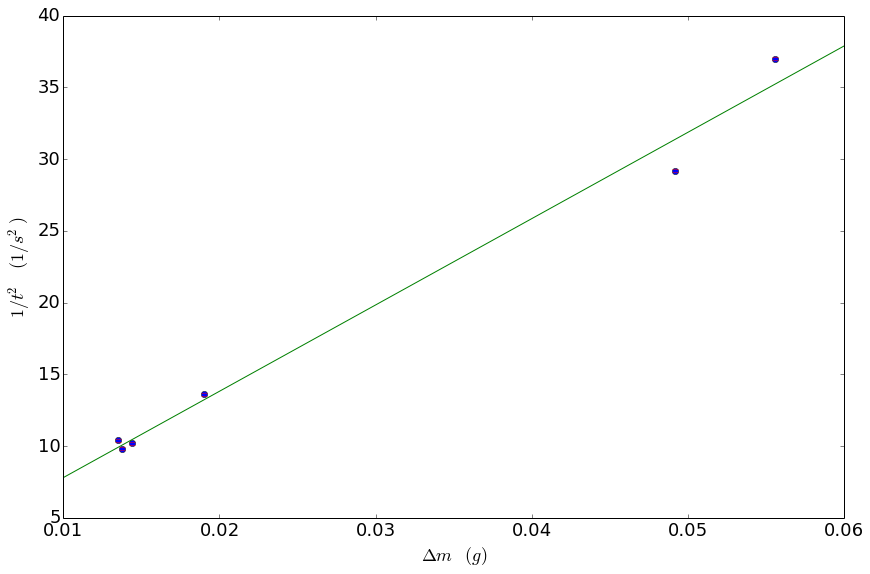
\includegraphics[scale=0.55]{grafico.png}
\caption{Regressão linear de $\Delta m$ por $1/t^2$ sobreposta aos pontos experimentais}
\label{grafico}
\end{figure}

\subsection{Significado do coeficiente angular}
O momento de inércia da polia de latão pode ser escrito em função do coeficiente angular $a$ pela fórmula 
$$I = a\cdot\frac{gR^2}{2h}-MR^2,$$
$$\Delta I = \sqrt{\Delta a^2 \cdot \frac{g^2R^4}{4h^2} + \Delta R^2 \cdot (a\frac{g}{h^2} - M)^2 + \Delta M^2\cdot R^4}$$
Sendo $\Delta I$ o erro da polia.
Assim, obtemos o valor do momento de inércia de 
$$ I = 0.00267 \pm 0.00004 \; Kg \cdot m^2 $$ 

\subsection{Significado do coeficiente linear}
Da equação linearizada original, vemos que o coeficiente linear é 
$$ b = \frac{\tau_a}{gR} $$
logo 
$$ \tau_a = bgR $$
$$ \Delta \tau_a = \sqrt{(gR \cdot \Delta b)^2 + (bg \cdot \Delta R)^2} $$
Assim, podemos calcular o valor de $\tau_a$ como 
$$ \tau_a =  0.00104 \pm 0.00004 \; N \cdot m $$

\section{Conclusões}




\end{document}

